% ***********************************************************
% ******************* PHYSICS HEADER ************************
% ***********************************************************
% Version 2
\documentclass[11pt]{article} 
\usepackage{amsmath} % AMS Math Package
\usepackage{amsthm} % Theorem Formatting
\usepackage{amssymb}	% Math symbols such as \mathbb
\usepackage{graphicx} % Allows for eps images
\usepackage{multicol} % Allows for multiple columns
\usepackage[dvips,letterpaper,margin=0.75in,bottom=0.5in]{geometry}
 % Sets margins and page size
\pagestyle{empty} % Removes page numbers
\makeatletter % Need for anything that contains an @ command 
\renewcommand{\maketitle} % Redefine maketitle to conserve space
{ \begingroup \vskip 10pt \begin{center} \large {\bf \@title}
	\vskip 10pt \large \@author \hskip 20pt \@date \end{center}
  \vskip 10pt \endgroup \setcounter{footnote}{0} }
\makeatother % End of region containing @ commands
\renewcommand{\labelenumi}{(\alph{enumi})} % Use letters for enumerate
% \DeclareMathOperator{\Sample}{Sample}
\let\vaccent=\v % rename builtin command \v{} to \vaccent{}
\renewcommand{\v}[1]{\ensuremath{\mathbf{#1}}} % for vectors
\newcommand{\gv}[1]{\ensuremath{\mbox{\boldmath$ #1 $}}} 
% for vectors of Greek letters
\newcommand{\uv}[1]{\ensuremath{\mathbf{\hat{#1}}}} % for unit vector
\newcommand{\abs}[1]{\left| #1 \right|} % for absolute value
\newcommand{\avg}[1]{\left< #1 \right>} % for average
\let\underdot=\d % rename builtin command \d{} to \underdot{}
\renewcommand{\d}[2]{\frac{d #1}{d #2}} % for derivatives
\newcommand{\dd}[2]{\frac{d^2 #1}{d #2^2}} % for double derivatives
\newcommand{\pd}[2]{\frac{\partial #1}{\partial #2}} 
% for partial derivatives
\newcommand{\pdd}[2]{\frac{\partial^2 #1}{\partial #2^2}} 
% for double partial derivatives
\newcommand{\pdc}[3]{\left( \frac{\partial #1}{\partial #2}
 \right)_{#3}} % for thermodynamic partial derivatives
\newcommand{\ket}[1]{\left| #1 \right>} % for Dirac bras
\newcommand{\bra}[1]{\left< #1 \right|} % for Dirac kets
\newcommand{\braket}[2]{\left< #1 \vphantom{#2} \right|
 \left. #2 \vphantom{#1} \right>} % for Dirac brackets
\newcommand{\matrixel}[3]{\left< #1 \vphantom{#2#3} \right|
 #2 \left| #3 \vphantom{#1#2} \right>} % for Dirac matrix elements
\newcommand{\grad}[1]{\gv{\nabla} #1} % for gradient
\let\divsymb=\div % rename builtin command \div to \divsymb
\renewcommand{\div}[1]{\gv{\nabla} \cdot #1} % for divergence
\newcommand{\curl}[1]{\gv{\nabla} \times #1} % for curl
\let\baraccent=\= % rename builtin command \= to \baraccent
\renewcommand{\=}[1]{\stackrel{#1}{=}} % for putting numbers above =
\newtheorem{prop}{Proposition}
\newtheorem{thm}{Theorem}[section]
\newtheorem{lem}[thm]{Lemma}
\theoremstyle{definition}
\newtheorem{dfn}{Definition}
\theoremstyle{remark}
\newtheorem*{rmk}{Remark}

% ***********************************************************
% ********************** END HEADER *************************
% ***********************************************************
\usepackage{cancel}
\usepackage{enumerate}
\usepackage{appendix}
\usepackage{pdfpages}
\usepackage{enumerate}
\title{Comp 350 Assignment 4}
\author{Ian Benlolo 260744397\\McGill University \\}
\begin{document}
\maketitle

\begin{enumerate}[1.]
\item
	\begin{enumerate}[(a)]
	\item We start by considering the taylor series of $f(c)$ around $c_n$ and $f[c_n+f(c_n)]$ around $c_n$:
	$$f(c)=f(c_n)+f'(c_n)(c-c_n)+\frac{f''(z)}{2}{(c-c_n)}^2 ,$$\\
	$$f[c_n+f(c_n)]=f(c_n)+f'(c_n)f(c_n)+\frac{f''(X_n)}{2}{f(c_n)}^2$$, 
	where $X_n$ is a point between $c_n$ and $c_n+f(c_n)$. Moving the latter around we get the following:
	$$\frac{f[c_n-f(c_n)]}{{f(c_n)}^2}=\frac{f'(c_n)+\frac{f''(X_n)f(c_n)}{2}}{f(c_n)}$$\\
	Taking the inverse and then forming the difference $c-c_{n+1}=c-c_n+\frac{f(c_n)}{f'(c_n)+\frac{f''(X_n)}{2}f(c_n)} = \frac{f(c_n)+f'(c_n)(c-c_n)+\frac{f''(X_n)}{2}f(c_n)(c-c_n)}{f'(c_n)+\frac{f''(X_n)}{2}f(c_n)}$.
	Taking the expansion of $f(c)$ around $c_n$, we can shorten it to $$f(c)=f(c_n)+f'(z*)(c-c_n)$$ where $z*$ does not necessarily equal $z$ or $X_n$. 
	Combining these and simplifying we get the following:$$c-c_{n+1}=-\frac{\frac{f''(z)}{2}{(c-c_n)}^2+\frac{f''(X_n)}{2}f'(z*){(x-x_n)^2}}{f'(c_n)+\frac{f''(X_n)}{2}f(c_n)}$$
	Using the fact the $f'(x)$ and $f''(x)$ are continuous; taking the limit of this we get:$$\lim_{n \to \infty}\frac{|c-c_{n+1}|}{|c-c_n|^2}=\lim_{n \to \infty}\left|{\frac{\frac{f''(z)}{2}+\frac{f''(X_n)}{2}f'(z*)}{f'(c_n)+\frac{f''(X_n)}{2}f(c_n)}}\right|=\frac{1}{2}\left|\frac{f''(c)}{f'(c)}\right||1+f'(c)|$$
	Since $f''(c)$ and $f'(c)$ are both continuous, this is equal to a constant. So this shows that the convergence is indeed quadratic unless $\frac{1}{2}\left|\frac{f''(c)}{f'(c)}\right||1+f'(c)|=0$ when the order is higher.
	
	
	\item The output of all my programs are attached at the bottom of this document. All three of the functions (newtons, secant and steffensen) found the correct answer of $2.1746$ but what is interesting is how many steps it took each and how costly they are and why. \\
	Newton's method was the fastest with $7$ iterations for $x_0=3$ and $6$ with $x_0=2.5$ which is expected because it computes $df$ separately, though this is inconvenient, quite costly sometimes and may not always be possible. Steffensen method, is a derivative of Newton's method because it replaces the derivative calculation with a forward difference approximation to it and can therefore be used to find roots of any function. It is more costly though because since calculating $f(x)$ and $f(x+h)$ are required. Steffensen's takes more steps than newton's method because the forward approximation uses a small interval  at each iteration which is correlated to $f(x)$, quadratically as proved above.\\
	The secant method is slower than newton's because it does not need to compute $fd$. It is faster than the steffenson method because it uses super-linear convergence.
	
	
	\end{enumerate}

%%question 2
\item 

From Newton's method, we know that $x_{i+1}=x_i-\frac{f(x_i)}{f'(x_i)}$ and $y_{i+1}=y_i-\frac{g(y_i)}{g'(y_i)}$. 

Expanding both $f(x,y)$ and $g(x,y)$ around $(x_0,y_0)$we  get $$f(x,y)=f(x_0,y_0)+(x-x_0)f_x+(y-y_0)f_y$$ and $$g(x,y)=g(x_0,y_0)+(x-x_0)g_x+(y-y_0)g_y$$
This can be generalized with the following function:$$f_{i+1}=f_i+(x_{i+1}-x_i)f_x+(y_{i+1}-y_i)f_y$$
This can also be done for $g(x,y)$.\\
Equating this to zero (since they converge to $0$) and rearranging, we get $$f_xx_{i+1}+f_yy_{i+1}=-f_i+x_if_x+f_yy_i,$$ 
$$g_xx_{i+1}+g_yy_{i+1}=-g_i+x_ig_x+y_ig_y$$
After solving for $x_{i+1}-x_i$ in both equations, we get $$x_{i+1}-x_i=\frac{-f_i-(y_{i+1}-y_i)f_y}{f_x}=\frac{-g_i-(y_{i+1}-y_i)g_y}{g_x}$$
$$\Rightarrow -f_xg_i-f_x(y_{i+1}-y_i)g_y=-g_xf_i-g_x(y_{i+1}-y_i)f_y$$
$$\Rightarrow (y_{i+1}-y_i)(f_yg_x-f_xg_y)=-g_xf_i+f_xg_i\Rightarrow y_{i+1}-y_i=\frac{f_xg_i-g_xf_i}{f_yg_x-f_xg_y}$$
and similarly, $$x_{i+1}-x_i=\frac{f_ig_y-g_if_y}{f_yg_x-f_xg_y}$$
which are equivalent to the formulas in question. 

\end{enumerate}

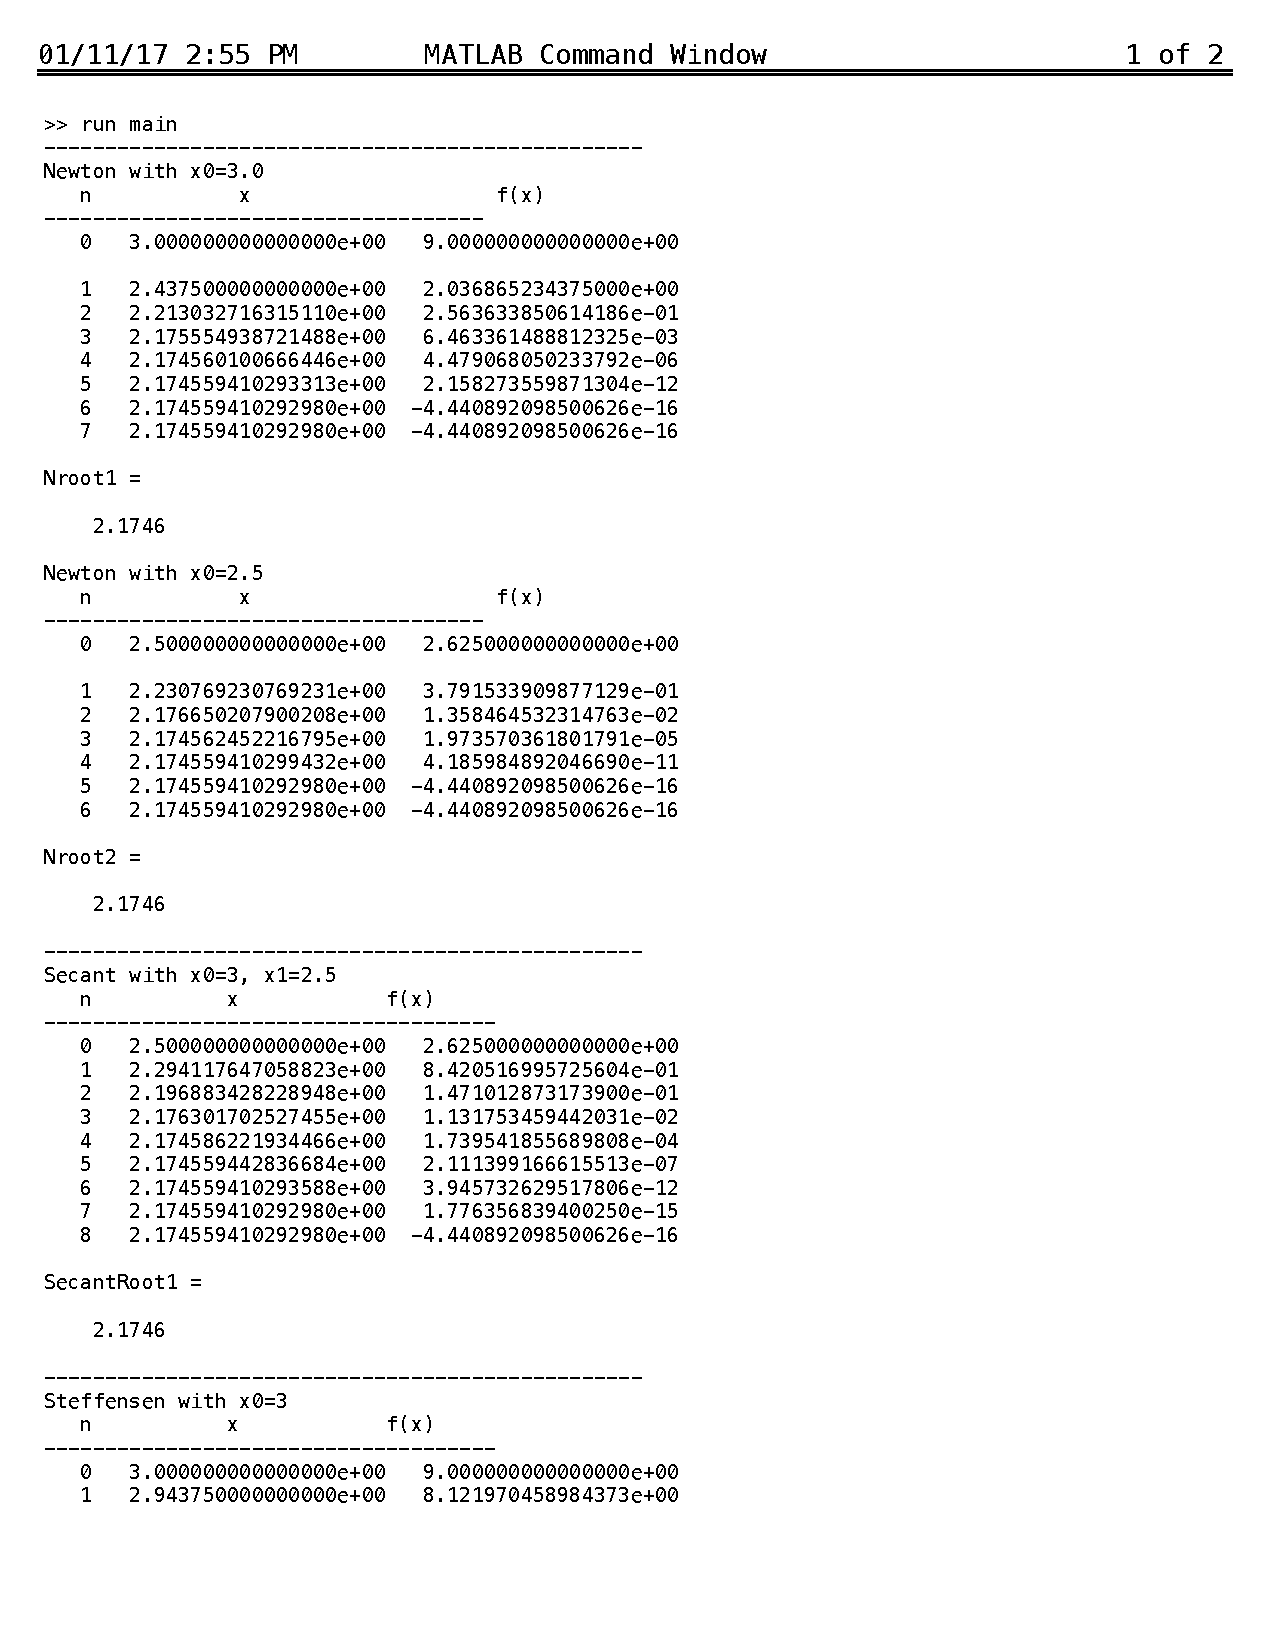
\includepdf[pages=-2]{output.pdf}


\end{document}